\section{\textsc{Vinaigrette}}

\subsection*{Ingredients for 100ml:}

\begin{tabular}{p{7.5cm} p{7.5cm}}
	& \\
	25ml vinegar & salt, pepper \& sugar \\
	75ml oil & 
\end{tabular}

\subsection*{Serving suggestion:}

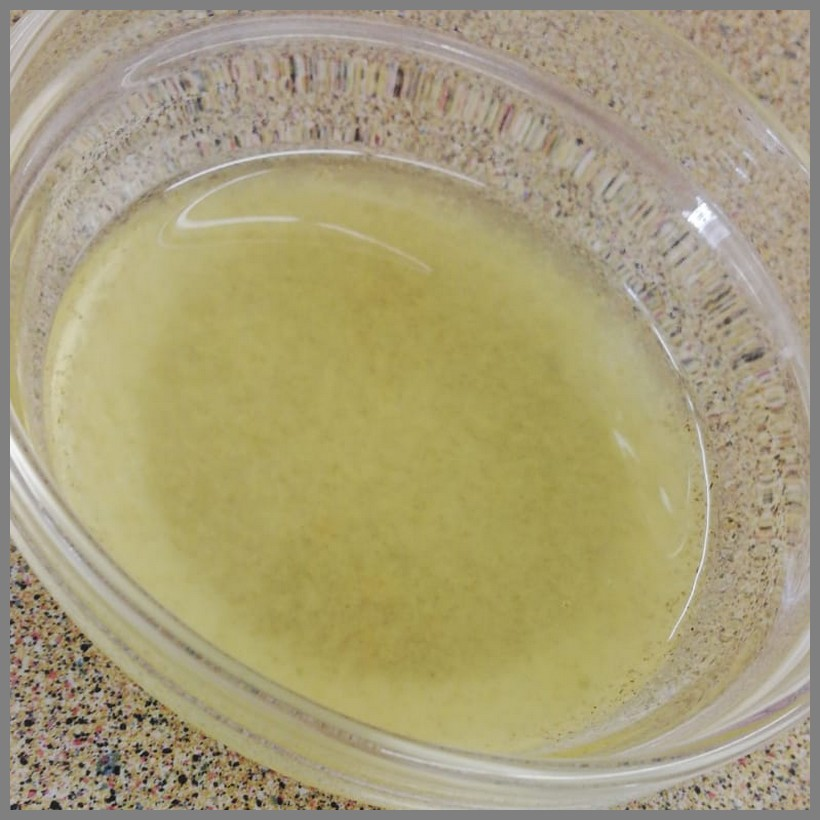
\includegraphics[width=\textwidth]{img/d_vinaigrette.jpeg} \cite{vinaigrette}

\subsection*{How it's done:}

\begin{tabular}{p{15cm}}
	\\
	Dissolve the salt in the vinegar, add the oil.\\
	Season it with pepper and finish it with sugar.\\
	\textbf{Tip:} You can use lemon or lime juice instead of vinegar.\\
	\\
	Suitable for all kinds of salad.
\end{tabular}
